\documentclass[11pt]{article}
\usepackage[english]{babel}
\usepackage{amsmath,amsthm,amsfonts,amssymb,epsfig}
\usepackage[left=1.1in,top=1in,right=1.1in]{geometry}
\usepackage{url}
\usepackage{array}
\usepackage{datetime}
\usepackage{lipsum}
\usepackage{url}
\usepackage{spverbatim}
\usepackage{paralist}
\usepackage{hyperref}
\hypersetup{colorlinks, urlcolor={blue}}
\usepackage{graphicx}
\graphicspath{ {images/} }
\newcommand{\argmin}{\operatornamewithlimits{argmin}}
\newcommand{\argmax}{\operatornamewithlimits{argmax}}


\begin{document}

\thispagestyle{empty} %removes page number

\begin{center}
\textsc{\Large\bf{Generalized Linear Modeling  with H2O's R Package}}
\\
\bigskip
\textsc{November 2014}
\end{center}
\bigskip
\bigskip 
\bigskip
\bigskip
\tableofcontents

\newpage

\section{Introduction} \label{1}
This document describes Generalized Linear Model implementation on H2O platform, list of supported features and how to use them from R. 

\section{What is H2O?}

H2O is fast scalable open -source machine learning and deep learning for Smarter Applications. With H2O enterprises like PayPal, Nielsen, Cisco and others can use all of their data without sampling and get accurate predictions faster. Advanced algorithms, like Deep Learning, Boosting and Bagging Ensembles are readily available for application designers to build smarter applications through elegant APIs. Some of our earliest customers have built powerful domain-specific predictive engines for Recommendations, Customer Churn, Propensity to Buy, Dynamic Pricing and Fraud Detection for the Insurance, Healthcare, Telecommunications, AdTech,
Retail and Payment Systems.

Using in-memory compression techniques, H2O can handle billions of data rows in-memory — even with a fairly small cluster. The platform includes interfaces for R, Python, Scala, Java, JSON and Coffeescript/JavaScript, along with its built-in Flow web interface that make it easier for non-engineers to stitch together complete analytic workflows. The platform was built alongside (and on top of) both Hadoop and Spark Clusters and is typically deployed within minutes.

H2O implements almost all common machine learning algorithms — such as generalized linear modeling (linear regression, logistic regression, etc.), Na\"{i}ve Bayes, principal components analysis, time series, k-means clustering and others. H2O also implements best-in-class algorithms such as Random Forest, Gradient Boosting and Deep Learning at scale. Customers can build thousands of models and compare them to get the best prediction results.

H2O is nurturing a grassroots movement of physicists, mathematicians, computer and data scientists to herald the new wave of discovery with data science. Academic re- searchers and Industrial data scientists collaborate closely with our team to make this possible. Stanford university giants Stephen Boyd, Trevor Hastie, Rob Tibshirani advise the H2O team to build scalable machine learning algorithms. With 100s of meetups over the past two years, H2O has become a word-of-mouth phenomenon growing amongst the data community by a 100-fold and is now used by 12,000+ users, deployed in 2000+ corporations using R, Python, Hadoop and Spark.

\textbf{Try it out}

H2O offers an R package that can be installed from CRAN. H2O can be downloaded from \url{www.h2o.ai/download}.

\textbf{Join the community}

Connect with \url{h2ostream@googlegroups.com} and \url{https://github.com/h2oai} to learn about our meetups, training sessions, hackathons, and product updates.

\textbf{Learn more about H2O}

Visit \url{www.h2o.ai}

\subsection{What is GLM?}
Generalized linear models (GLM) are the workhorse for most predictive analysis use cases. GLM can be used for both regression and classification, it scales well to large datasets and is based on solid statistical background. It is a generalization of linear models, allowing for modeling of data with exponential distributions and for categorical data (classification). GLM models are fitted by solving the maximum likelihood optimization problem.

\subsection{GLM on H2O}
H2O's GLM algorithm fits the generalized linear model with elastic net penalties. The model fitting computation is distributed, extremely fast, and scales extremely well for models with a limited number (~ low thousands) of predictors with non-zero coefficients. The algorithm can compute models for a single value of a penalty argument or the full regularization path, similar to glmnet package for R\cite{glmnet}. 
H2O's GLM fits the model by solving following problem:

\[ \min\limits_{\beta}\ {{1\over{N}} log-likelihood(family,\beta)  + \lambda (\alpha \| \beta \|_1}  + {1- \alpha \over 2} \| \beta \|_2^2) \]

The elastic net parameter $\alpha$ controls the penalty distribution between L1 and L2 penalty. It can have any value between 0 and 1. When $\alpha$ = 0, we have no L1 penalty and the problem becomes ridge regression. If $\alpha$ = 1, there is no L2 penalty and we have lasso.

The main advantage of an L1 penalty is that with sufficiently high $\lambda$, it produces a sparse solution; the L2-only penalty does not reduce coefficients to exactly 0. The two penalties also differ in the case of correlated predictors. The L2 penalty shrinks coefficients for correlated columns towards each other, while the L1 penalty will pick one and drive the others to zero. Using the elastic net argument $\alpha$, you can combine these two behaviors. It is also useful to always add a small L2 penalty to increase numerical stability.

Similarly to \cite{glmnet}, H2O can compute the full regularization path, starting from null-model (maximum penalty) going down to minimally penalized model. This search is made efficient by employing strong-rules \cite{strong} to filter out inactive coefficients (coefficients pushed to zero by penalty). Computing full regularization path is useful in that it gives more insight about the importance of individual coefficients and quality of the model while allowing selection of the optimal amount of penalization for the given problem and data.


\subsubsection{Summary of features} 
In summary, H2O's GLM functionalities include:

\begin{itemize} 
\item fits generalized linear model with elastic net penalty
\item supported GLM families include Gaussian, Binomial, Poisson and Gamma
\item efficient handling of categorical variables
\item efficient computation full regularization path
\item efficient distributed n-fold cross validation
\item distributed grid search over elastic-net parameter $\alpha$
\item upper and lower bounds for coefficients
\item proximal operator interface
\end{itemize}



\section{Installation} 

You can load the latest CRAN H2O package by running:

\begin{spverbatim}
> install.packages("h2o")
\end{spverbatim}
\bigskip
\noindent
Alternatively, you can (and should for this tutorial) download the latest H2O build by following the ``Install in R" instructions in the H2O download table:

\indent \indent \indent \url{http://s3.amazonaws.com/h2o-release/h2o/master/latest.html}.

\noindent
Open your R Console and run the following to install the latest H2O build in R:

\begin{spverbatim}
# The following two commands remove any previously installed H2O packages for R.
> if ("package:h2o" %in% search()) { detach("package:h2o", unload=TRUE) }
> if ("h2o" %in% rownames(installed.packages())) { remove.packages("h2o") }

# Next, we download, install and initialize the H2O package for R
# replace the *s below with the release number found on our download page
> install.packages("h2o", repos=(c("http://s3.amazonaws.com/h2o-release/h2o/
master/****/R", getOption("repos"))))

# Load h2o library in R
> library(h2o)

\end{spverbatim}
\noindent
To launch on a single node, initialize H2O on all the cores of your machine with

\begin{spverbatim}
> localH2O = h2o.init(nthreads = -1)

\end{spverbatim}
\noindent
The function \texttt{h2o.init()} will initialize a H2O instance and instantiates a H2O client module. By default, the H2O instance will launch on \texttt{localhost:54321}. To establish a connection to an existing H2O cluster node, explicitly state the IP address (\texttt{ip = "localhost"}) and port number (\texttt{port = 54321}) in the \texttt{h2o.init()} call.

\noindent
Run the following command to observe an example classification model built through H2O's GLM:

\begin{spverbatim}
# Build a GLM model on prostate data with formula: CAPSULE ~ AGE + RACE + PSA + DCAPS
> prostatePath = system.file("extdata", "prostate.csv", package = "h2o")
> prostate.hex = h2o.importFile(localH2O, path = prostatePath, key = "prostate.hex")
> h2o.glm(y = "CAPSULE", x = c("AGE","RACE","PSA","DCAPS"), data = prostate.hex, family = "binomial", nfolds = 0, alpha = 0.5, lambda_search = FALSE,  
use_all_factor_levels = FALSE, variable_importances = FALSE, higher_accuracy = FALSE)
\end{spverbatim}

\vspace{10 mm}
\noindent
The output of the model build will include coefficients, as well as some validation statistics:

\begin{spverbatim}       
IP Address: 127.0.0.1 
Port      : 54321 
Parsed Data Key: prostate.hex 

GLM2 Model Key: GLMModel__827586bb2c59ba79dc129b8500174940

Coefficients:
      AGE      RACE     DCAPS       PSA Intercept 
 -0.01104  -0.63136   1.31888   0.04713  -1.10896 

Normalized Coefficients:
      AGE      RACE     DCAPS       PSA Intercept 
 -0.07208  -0.19495   0.40972   0.94253  -0.33707 

Degrees of Freedom: 379 Total (i.e. Null);  375 Residual
Null Deviance:     512.3
Residual Deviance: 449.5  AIC: 459.5
Deviance Explained: 0.12254 
 Best Threshold: 0.28

Confusion Matrix:
        Predicted
Actual   false true Error
  false     75  152 0.670
  true      18  135 0.118
  Totals    93  287 0.447

AUC =  0.7157151 (on train)
\end{spverbatim}

\subsection{Support} 

Users of the H2O package may submit general enquiries and bug reports privately to H2O via email: \url {support@h2o.ai}; or publicly post them to: \url {h2ostream@googlegroups.com}. Specific bugs or issues will be filed to H2O's JIRA: 
\url{https://0xdata.atlassian.net/secure/Dashboard.jspa}.

\section{Generalized Linear Modeling} 
This section contains a brief overview of generalized linear models and follows up with a few details for each model family.

Generalized linear models are generalization of linear regressions. Linear regression models the dependency of response y on a vector of predictors x ($y \sim x^T \beta + \beta_0$). The models are built with the assumptions that y has a gaussian distribution with a variance of $\sigma^2$ and the mean is a linear function of x with an offset of some constant $\beta_0$, i.e. $ y = \mathcal{N}(x^T \beta + \beta_0 ,  \sigma^2) $. These assumptions can be overly restrictive for real-world data that do not necessarily follow have a gaussian distribution. GLM generalizes linear regression in the following ways: 
\begin{itemize} 
\item adds a non-linear link function that transforms the expectation of response variable, so that $link(y) \sim x^T \beta + \beta_0$.
\item allows variance to depend on the predicted value by specifying the conditional distribution of the response variable or the family argument.

\end{itemize}
This generalization allows us to use GLM on problems such as binary classification (Logistic regression).

\subsubsection{Model Fitting}
GLM models are fitted by maximizing the likelihood. For the gaussian family, maximum likelihood is simply the minimal mean squared error, which has an analytical solution and can be solved with ordinary least squares. For all other families, the maximum likelihood problem has no analytical solution so we must use an iterative method such as IRLSM, Newton method, gradient descent, and L-BFGS.
\subsubsection{Model Validation}
Evaluating the quality of the model is a critical part of any data-modeling and scoring process. There are several standard ways on how to evaluate the quality of the fitted GLM model; the most common method is to use the resulting deviance. Deviance is calculated by comparing the log likelihood of the fitted model with log likelihood of the saturated model (or theoretically perfect model).

\[ deviance = 2({ln(L_{s})} - {ln(L_{m})}) \]

Another metric frequently used for model selection is the Akaike information criterion (AIC). AIC is a measure of the relative quality of a statistical model for a given set of data that is obtained by calculating the information loss when replacing the original data with the model itself. Unlike deviance, which would assign a perfect value for the saturated model and measures the absolute quality of the fit with a comparison against the null-hypothesis, it takes into account the complexity of the given model. AIC is defined as follows:

\[ aic = 2(k - ln(L_{m}))\]

\noindent
where k is the number of model parameters and $ln(L_{m})$ is the log likelihood of the fitted model over the data.


\subsection{Regularization} 
We introduce penalties to model-fitting to avoid over-fitting, reduce variance of the prediction error, and deal with correlated predictors. There are two common penalized linear models: Ridge Regression and Lasso. Ridge regression provides greater numerical stability and is easier (faster) to compute. On the other hand, Lasso leads to a sparse solution, which is a big advantage in many situations, as it can be used for feature selection and to produce models with fewer parameters. When encountering highly correlated columns, the L2 penalty tends to push all of the coefficients towards each other, while the L1 penalty will pick one and remove the others (0 coefficients).

\subsubsection{Lasso}

Lasso represents the L1 penalty and is an alternative regularized least squares method that uses the constraint $||B||_1$. The penalty is configured using the \texttt{alpha} parameter. The main difference between lasso and ridge regression is that as the penalty for ridge regression increases, the parameters are reduced to non-zero values. With lasso, if the penalty is increased, the parameters can be reduced to zero values. Since reducing parameters to zero removes them from the model, the lasso method provides only the relevant data. Ridge regression never removes any data. 

\subsubsection{Elastic Net Penalty}

H2O supports elastic net regularization which is parametrized by \textit{alpha} and \textit{lambda} arguments (similarly to \cite{glmnet})

The \textit{alpha} argument controls the elastic net penalty distribution to L1 and L2 norms. It can have any value in [0,1] range (inclusive) or a vector of values (triggers grid search). Alpha = 0 leads to \textbf{Ridge Regression}, alpha = 1 leads to \textbf{LASSO}.  

The \textit{lambda} argument controls the penalty strength; it can have any positive value or a vector of values (which triggers grid search).
\textbf{Note:} Lambda values are capped at $\lambda_{max}$, which is the smallest $\lambda$ s.t. the solution is empty model (all zeros except for intercept).

Elastic net combines the two and adds another parameter, $\alpha$, which controls distribution of the penalty between L1 and L2. The combination of the two penalties is beneficial, since L1 gives sparsity while L2 gives stability and encourages the grouping effect (where a group of correlated variables tends to be dropped or added into the model all at once).One possible use of the $\alpha$ argument is to do lasso with very little L2 penalty ($\alpha$ almost 1) to stabilize the computation (improve convergence speed)

Model-fitting problem with elastic net penalty becomes:

\[ \min\limits_{\beta,\beta_0}\ {{1\over{N}} ln(L(family,\beta,\beta_0))  + \lambda (\alpha \| \beta \|_1}  + {1- \alpha \over 2} \| \beta \|_2^2) \]


\subsection{GLM Models} 
The following subsection describes GLM families supported in H2O. 

\subsubsection{Linear Regression (Gaussian family) }
Linear regression refers to the gaussian family model. It is the simplest example of GLM, but it has many uses and several advantages over the other families, such as faster and more stable computation. 

It models the dependency as a purely linear function (with link = identity):
\[ \hat{y} = x^T\beta + \beta_0\]

The model is fitted by solving the least squares problem (maximum likelihood for gaussian family):

\[ \min\limits_{\beta,\beta_0} { {1 \over 2N}\sum\limits_{i=1}\limits^{N}(x_i^{T}\beta  + \beta_0- y_i)^T (x_i^{T}\beta + \beta_0 - y_i)  + \lambda (\alpha \|\beta \|_1 + {1-\alpha \over 2}) \| \beta \|_2^2} \]


Deviance is simply the sum of squared errors:
\[ D = \sum\limits_{i=1}\limits^{N}{(y_i - \hat{y}_i)^2} \]


\textbf{Example}\\
Included in the H2O package is a prostate cancer data set. The data was collected for a study done by Dr. Donn Young at The Ohio State University Comprehensive Cancer Center of patients with varying degrees of prostate cancer. Below a model is built to predict the volume (VOL) of tumors obtained from ultrasounds based on features such as age and race.

\begin{spverbatim}
> filepath = system.file("extdata", "prostate.csv",package = "h2o")
> prostate.hex = h2o.importFile(object = localH2O, filepath, key = "prostate.hex")
> gaussian.fit = h2o.glm(x = c("AGE", "RACE", "PSA", "GLEASON"), y = "VOL", data = prostate.hex, family = "gaussian")
\end{spverbatim}

\subsubsection{Logistic Regression (Binomial Family)}
Logistic regression can be used in case of a binary classification problem, where the response is categorical with two levels. It models dependency as $Pr(y = 1|x)$. The canonical link for binomial family is logit (log of the odds) and its inverse is a logistic function that takes any real number on the input and projects it onto the 0,1 range (s-curve).  The s-curve is shown below: 

\begin{figure}[h]
\centering
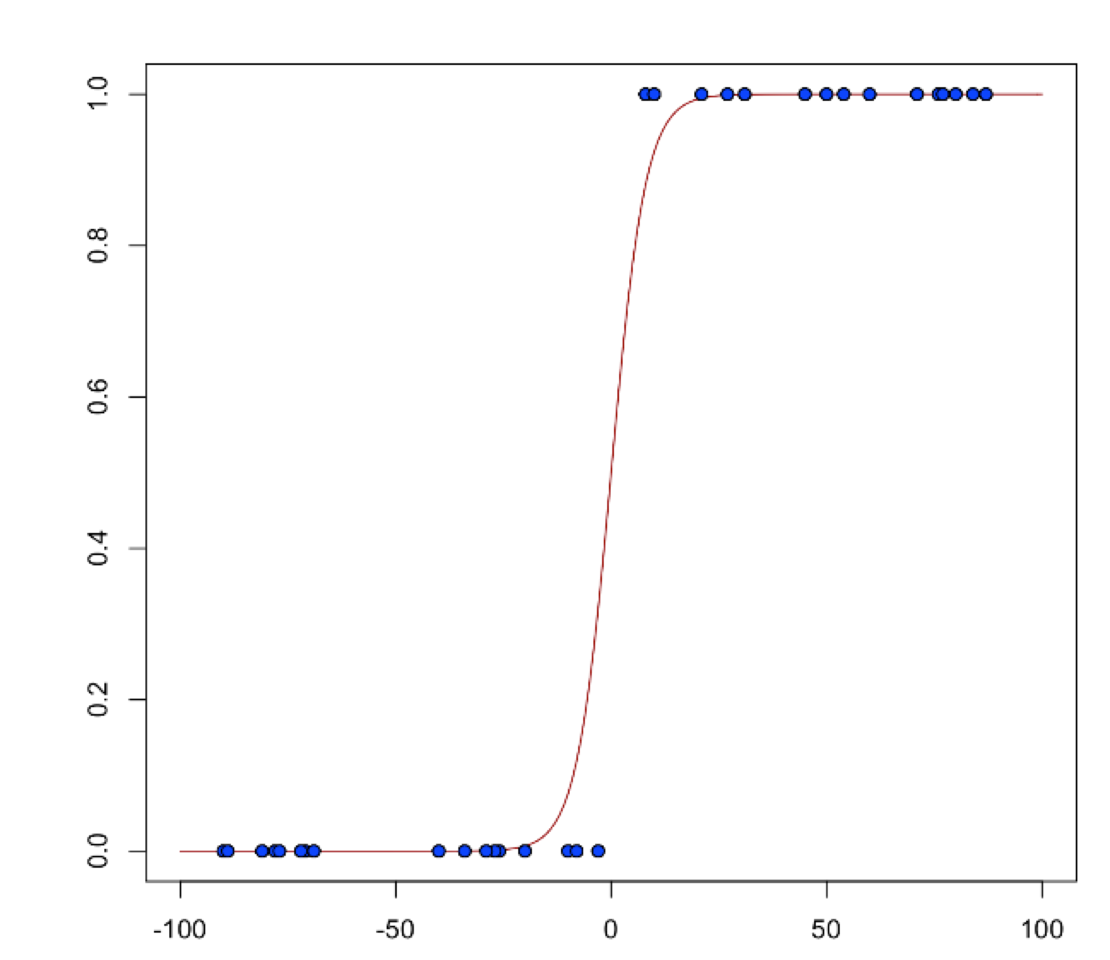
\includegraphics[scale=0.5]{scurve.png}
\end{figure}


 

\[ \hat{y} = Pr(y = 1|x) = {e^{x^T\beta + \beta_0} \over 1 + e^{x^T \beta + \beta_0} } \]

or alternatively:


\[log {\hat{y} \over 1- \hat{y}} = log{Pr(y=1|x) \over Pr(y=0|x)} = x^T \beta + \beta_0\]

The model is fitted by solving:
\[  \min\limits_{\beta,\beta_0} { {1 \over N}\sum\limits_{i=1}\limits^{N}(y_i (x_i^{T}\beta  + \beta_0) - log (1 + e^{x_i^{T}\beta  + \beta_0} )  + \lambda (\alpha \|\beta \|_1 + {1-\alpha \over 2}) \| \beta \|_2^2} \]

Deviance is -2 log likelihood:
\[D = -2\sum\limits_{i=1}\limits^{N}{(y log(\hat{y}) + (1 - y)log(1-\hat{y})  )}\]

\textbf{Example}\\
Using the prostate data set, build a binomial model that classifies if there is penetration of the prostatic capsule (CAPSULE). Make sure the entries in the CAPSULE column are binary entries by using the \texttt{h2o.table()} function. Change the regression by setting the family to binomial.
\begin{spverbatim}
> h2o.table(prostate.hex[,"CAPSULE"])
  row.names Count
1         0   227
2         1   153
> binomial.fit = h2o.glm(x = c("AGE", "RACE", "PSA", "GLEASON"), y = "CAPSULE", data = prostate.hex, family = "binomial")
\end{spverbatim}

\subsubsection{Poisson Models}
Poisson regression is generally used in cases where the response represents counts and we assume errors have a Poisson distribution. In general, it can be applied to any data where the response is non-negative. 

When building a Poisson model, we usually model dependency of the mean on the log scale, i.e. canonical link is log and prediction is:

\[\hat{y} = e^{x^T\beta + \beta_0}\]

The model is fitted by solving:

\[  \min\limits_{\beta,\beta_0} { {1 \over N}\sum\limits_{i=1}\limits^{N}(y_i (x_i^{T}\beta  + \beta_0) - e^{x_i^{T}\beta  + \beta_0})  + \lambda (\alpha \|\beta \|_1 + {1-\alpha \over 2}) \| \beta \|_2^2} \]

Deviance is 

\[D = -2\sum\limits_{i=1}\limits^{N}{(y log(\hat{y}) - y - \hat{y}}\]


\textbf{Example}\\
Load the Insurance data from the MASS library and import into H2O. Run a poisson model that predicts the number of claims (Claims) based on the district of the policy holder (District), their age (Age), and the type of car they own (Group).
\begin{spverbatim}
> library(MASS)
> data(Insurance)
> insurance.hex = as.h2o(localH2O, Insurance)
> poisson.fit = h2o.glm(x = c("District", "Group", "Age"), y = "Claims", 
data = insurance.hex, family = "poisson")
\end{spverbatim}

\subsubsection{Gamma Models}
The gamma distribution is useful for modeling a positive continuous response variable, where the conditional variance of the response grows with its mean but  the coefficient of variation of the response $\sigma^2(x)/μ(x)$ is constant for all x,  i.e., it has a constant coefficient of variation.

It is usually used with inverse or log link, inverse is the canonical link.

The model is fitted by solving:

\[  \min\limits_{\beta,\beta_0} { {1 \over N}\sum\limits_{i=1}\limits^{N}{y_i \over (x_i^{T}\beta  + \beta_0)} - log({x_i^{T}\beta  + \beta_0})  + \lambda (\alpha \|\beta \|_1 + {1-\alpha \over 2}) \| \beta \|_2^2} \]

Deviance is 

\[D = -2\sum\limits_{i=1}\limits^{N}{log({y_i \over \hat{y}_i}) - {y_i - \hat{y}_i \over\hat{y}_i }}\]


\textbf{Example}\\
To change the link function from the default inverse function to the log link function, modify the \textit{link} argument.

\begin{spverbatim}
> gamma.inverse <- h2o.glm(x=c("AGE","RACE","CAPSULE","DCAPS","PSA","VOL"), y="DPROS", data=prostate.hex, family="gamma", link="inverse")

> gamma.log <- h2o.glm(x=c("AGE","RACE","CAPSULE","DCAPS","PSA","VOL"), y="DPROS", data=prostate.hex, family="gamma", link="log")
\end{spverbatim}

% Strong Rules paper


\section{GLM on H2O}
This section describes the specifics of GLM implementation on H2O, such as selecting regularization parameters and handling of categoricals. 

H2O's GLM implementation presents a high-performance distributed algorithm, which scales linearly with the number of rows and works extremely well for datasets with limited number of active predictors. 

\subsection{Input Parameters}
\subsubsection{Predictors \& Response}
Every model must specify its predictors and response. It is the equivalent formula object in R. Predictors and response are specified by \textit{source} and \textit{x} and \textit{y} parameters, with an optional \textit{offset} parameter. 

\textit{source} refers to a frame containing a training dataset. All predictors and the response (and offset, if there is one) must be part of this frame.

\textit{x} contains the list of column names or column indices referring to vectors from the source frame; it can not contain periods.

\textit{y} is a column name or index referring to a vector from the source frame.

\textit{offset} is a column name or index referring to a vector from the source frame.
  
\subsubsection{Family \& Link}
Family and Link are both optional parameters. The default family is \textit{Gaussian} and the default link is a canonical link for the selected family. These are passed in as strings, e.g. \textit{family=`gamma', link = `log'}.
While it is possible to select something other than a canonical link, it can lead to an unstable computation. Recommended combinations are Gaussian and Log, or Inverse and Gamma with log.  



\subsubsection{Lambda-Search}
Lambda search is special case of automatic and efficient grid search over lambda argument and is described in its own section. Lambda search can be enabled by using the \textit{lambda\_search = T} option. It can be further parametrized by the \textit{n\_lambdas} and \textit{lambda\_min\_ratio} parameters. 
\textit{n\_lambdas} specifies the number of lambda values on the regularization path
\textit{lambda\_min\_ratio} specifies the minimal lambda value to be computed as a ration of $\lambda_{max}$

\subsection{Coefficient Constraints}
Coefficient constraints allow you to set special conditions over the model coefficients. Currently supported constraints are upper and lower bounds and proximal operator \cite{prox} interface. 

The constraints are specified as a frame with following vecs (matched by name, all vecs can be sparse):
\begin{itemize}
\item \textit{names (mandatory)}  - coefficient names. 
\item \textit{lower\_bounds (optional)} - coefficient lower bounds , must be $<= 0$
\item \textit{upper\_bounds (optional)} - coefficient upper bounds , must be $>= 0$
\item \textit{beta\_given (optional)} - specifies the given solution in proximal operator interface
\item \textit{rho (mandatory if beta\_given is specified, otherwise ignored)} - specifies per-column L2 penalties on the distance from the given solution
\end{itemize}
 
The proximal operator interface allows you to run the GLM with a proximal penalty on a distance from a specified given solution. It has various uses: for example, it can be used as part of ADMM consensus algorithm to obtain unified solution over separate H2O clouds, or in Bayesian regression approximation.

\subsection{H2O GLM Model Output}
The detailed output of the GLM model varies depending on the distribution used for the model. In general, there are common parts of the output for all Families: Coefficients \& Normalized Coefficients, Validation, and Prediction. We'll cover the model output from an R user's  point of view.

First, let's build a simple GLM on a small dataset and see what we get out:

\begin{verbatim}
library(h2o)

# instantiate h2o
h <- h2o.init()

# path to the data
# path is split up so it's document friendly
data.bucket <- "https://raw.githubusercontent.com/h2oai/h2o/master/smalldata"
data.path <- paste(data.bucket, "/logreg/prostate_train.csv", sep = "")

# import the data from the url
hex <- h2o.importFile(h, data.path)

# build a binomial regression
m <- h2o.glm(x = 3:9, y = 2, data = hex, family = "binomial")  # no other features tweaked... yet
\end{verbatim}

The default \texttt{show} of this model has the following output:

\begin{verbatim}
IP Address: 127.0.0.1 
Port      : 54321 
Parsed Data Key: prostate_train.hex 

GLM2 Model Key: GLMModel__8b954fd700d924f3e9dee8717b8246ef

Coefficients:
      AGE      RACE     DPROS     DCAPS       PSA       VOL   GLEASON Intercept 
 -0.07668  -0.10320   0.59479   0.13549   0.43841  -0.22215   1.19657  -0.49458 

Normalized Coefficients:
      AGE      RACE     DPROS     DCAPS       PSA       VOL   GLEASON Intercept 
 -0.07668  -0.10320   0.59479   0.13549   0.43841  -0.22215   1.19657  -0.49458 

Degrees of Freedom: 304 Total (i.e. Null);  297 Residual
Null Deviance:     412.1
Residual Deviance: 301.9  AIC: 317.9
Deviance Explained: 0.26733 
 Best Threshold: 0.44

Confusion Matrix:
        Predicted
Actual   false true Error
  false    147   34 0.188
  true      32   92 0.258
  Totals   179  126 0.216

AUC =  0.8318927 (on train) 
\end{verbatim}

Briefly, the output contains the IP address and port number of the H2O cluster where the model was trained. It includes the data key, the model key, the coefficients, and  some model metrics. Let's look at these more in-depth.

\subsubsection{Coefficients \& Normalized Coefficients}
\textit{Coefficients} are the predictor weights, i.e. the actual model used for prediction. 

If the \textit{standardize} option is set, H2O returns another set of coefficients, \textit{Normalized Coefficients}. These are the predictor weights of the standardized data and are included only for informative purposes (e.g. to compare relative variable importance). In this case, the \textit{Coefficients} are obtained from \textit{Normalized Coefficients} by \textbf{reversing} the data standardization process (de-scaled, intercept adjusted by added offset) so that they can be applied to data in its original form (i.e. no standardization prior to scoring). \textit{Note:} These are \textbf{not} the same as coefficients of a model built on non-standardized data.

\subsubsection{Validation}

H2O's GLM performs 10-fold cross-validation by default. It does this by generating additional models with 1/10 of the original data. This is fast and gives some idea of how the model will generalize. However, it's always best to evaluate the model using some holdout data.

\subsubsection{Generating Predictions}

The following R code generates predictions:

\begin{verbatim}
test.path <- paste(data.bucket, "/logreg/prostate_test.csv", sep = "")

# import the data from the url
test <- h2o.importFile(h, test.path)

# generate the predictions
predictions <- h2o.predict(m, test)

# look at the first 6 entries of predictions
predictions

# generate the model metrics
h2o.performance(data=predictions[,3], reference=test[,1])
\end{verbatim}


\subsection{Categorical Variables}
When applying linear models to datasets with categorical variables, the usual approach is to expand the categoricals into a set of binary vectors, with one vector per each categorical level (e.g. by calling {\texttt{model.matrix}} in R). H2O performs similar expansions automatically and no prior changes to the dataset are needed. Each categorical column is treated as a set of sparse binary vectors.

\subsubsection{Largest Categorical Trick}
Categoricals have special handling during GLM computation as well. When forming the gram matrix, we can exploit the fact that columns belonging to the same categorical never co-occur and the gram matrix region belonging to these columns will not have any non-zero elements outside of the diagonal. We can thus keep it in sparse representation taking only O(N) elements instead of O(N*N). Furthermore, the complexity of Choelsky decomposition of a matrix that starts with a diagonal region can be greatly reduced. H2O's GLM exploits these two facts to handle the largest categorical ``for free". Therefore, when analyzing the performance of GLM in the equation expressed above, we can subtract the size of the largest categoricals from the number of predictors.
\[ N = \sum\limits_{c \in C} (\|c.domain\|) - \argmax\limits_{c \in C} \|c.domain\|  + \| Nums \| \]

\subsection{Cross-Validation}
All validation values can be computed either on the training data set (the default) or using nfold cross-validation ($nfolds > 1$). When using nfold cross-validation, we randomly split data into n equally-sized parts and train each of the n models on n-1 parts and compute validation on the part which was not used for training.The reported validation parameters are then obtained as follows:
\begin{itemize} 
\item null deviance is sum of null deviances of n-models (each uses null model based on the subset of the data)
\item residual deviance is sum of residual deviances of all n-models.
\item AIC is based on log-likelihood, which is summed up similarly to deviance
\item AUC is based on ROC curve build  by summing up confusion matrices built for all n-models.
This means for each threshold, we get a confusion matrix that includes all the rows from
the training set. However, each row is classified exclusively by the model
that did not have it in its training set. The computation of AUC itself is then the same as in a non-cross-validated case. 
\end{itemize}

\subsection{Selecting Regularization Parameters}
To get the best possible model, we need to find the optimal values of the regularization parameters $\alpha$ and $\lambda$. 
To this end, H2O provides grid search over $\alpha$ and a special form of grid search called ``lambda search over $\lambda$". The recommended way to find optimal regularization settings on H2O is to do a grid search over a few $\alpha$ values with an automatic lambda search for each $\alpha$. Both are described below in greater detail. 
\subsubsection{Grid Search Over Alpha}
Alpha search is not always needed and simply changing its value to 0.5 (or 0 or 1 if we only want Ridge or Lasso, respectively) works in most cases. If $\alpha$ search is needed, usually only a few values are sufficient. Alpha search is invoked by supplying a list of values for $\alpha$ instead of a single value. H2O then produces one model per $\alpha$ value. The grid search computation can be done in parallel (depending on the cluster resources) and it is generally more efficient than computing different models separately from R. 

Use caution when including $\alpha=0$ or $\alpha=1$ in the grid search. $\alpha=0$ will produce a dense solution and it can be really slow (or even impossible) to compute in large N situations. $\alpha=1$ has no L2 penalty, so it is therefore less numerically stable and can be very slow as well due to slower convergence. In general, it is safer to run with $alpha=1-\epsilon$ instead.

\subsubsection{Lambda Search}
Lambda search can be enabled by using the \textit{lambda\_search = T} option. It can be further parametrized by the \textit{n\_lambdas} and \textit{lambda\_min\_ratio} parameters. When this option is enabled, H2O performs a specialized grid search over the list of \textit{n\_lambdas} $\lambda$ values, producing one model each per  $\lambda$ value. 

The $\lambda$-list is automatically generated as an exponentially decreasing sequence, going from $\lambda_{max}$,
the smallest $\lambda$ s.t.the solution is a model with all 0s, to $\lambda_{min} = $ \textit{lambda\_min\_ratio} * $ \lambda_{max}$.

H2O computes $\lambda$-models sequentially and in decreasing order, warm-starting the model for $\lambda_k$ with the solution for $\lambda_{k-1}$. By warm-starting the models, we get better performance: typically models for subsequent $\lambda$s are close to each other, so we need only a few iterations per $\lambda$ (typically 2 or 3). We also achieve greater numerical stability, since models with a higher penalty are easier to compute; so, we start with an easy problem and then keep making only small changes to it.

\textbf{Note:} \textit{nlambda}, \textit{lambda.min.ratio} also specify the relative distance of any two lambdas in the sequence. This is important for the application of recursive strong rules, which are only effective if the neighbouring lambdas are \textit{"close"} to each other. The default values are \textit{nlambda} = 100 and $\lambda_{min} = \lambda_{max} 1e^{-4}$, which gives us the ratio of 0.912.   In order for strong rules to work, you should keep the ratio close to the default.  
    
\subsubsection{Grid Search Over Lambdas}
While automatic lambda search is the preferred method, it is also possible to do a grid search over lambda values by passing in vector of lambdas and disabling the lambda-search option. The behavior will be identical to lambda search, except H2O will use a user-supplied list of lambdas instead (still capped at $\lambda_{max}$).

\subsection{Strong Rules} %TODO add references
H2O's GLM employs strong rules \cite{strong} to discard predictors that are likely to have 0 coefficients prior to model building. According to \cite{strong}, we can identify such predictors based on a gradient with great accuracy (very few false negatives and virtually no false positives in practice), greatly reducing the computational complexity of model fitting and enabling it to run on wide datasets with tens of thousands of predictors, provided that there is a limited number of active predictors. 

When applying the strong rules, we evaluate the gradient at the starting solution, filter out inactive coefficients, and fit a model using only a subset of the available predictors. Since strong rules may have false positives (which are extremely rare in practice), we need to check the solution by testing the kkt conditions and verify that all discarded predictors indeed have 0 coefficients.  

\subsection{Performance Characteristics}
The implementation is based on iterative reweighted least squares with ADMM \cite{admm} inner solver to deal with L1 penalty. Every iteration of the algorithm consists of following steps:
\begin{enumerate} 
\item Generate weighted least squares problem based on previous solution, i.e. vector of weights w and response z 
\item Compute the weighted gram matrix $X^TWX$ and $X^Tz$ vector
\item Decompose the gram matrix (Cholesky decomposition) and apply ADMM solver to solve the L1 penalized least squares problem
\end{enumerate}

Steps 1 and 2 are performed distributively and step 3 is computed in parallel on a single node. We can thus characterize the computational complexity and scalability of dataset with M observations and N columns (predictors) on a cluster with n nodes with p CPUs each as follows:

\[ O({MN^2 \over pn} + {N^3 \over p})\]

And the overall memory cost is given by:

\[ O(MN + N^2pn)\]

In case of $M >> N$, we can forget the second term and the algorithm scales linearly both in the number of nodes and number of CPUs per node. However, the equation above also implies that our algorithm is limited in the number of predictors it can handle, since the size of the Gram matrix grows quadratically (due to a memory and network throughput issue) with the number of predictors and its decomposition cost grows as the cube of the number of predictors (which is computational cost issue). H2O can get around these limitations in many cases due to its handling of categoricals and by employing strong rules to filter out inactive predictors; both are described later in this chapter.  


\section{Use case: Classification with Airline data}


\subsection{Airline dataset overview} 

The Airline dataset can be downloaded here: \url{https://github.com/h2oai/h2o/blob/master/smalldata/airlines/allyears2k_headers.zip}. Remember to save the .csv file to your working directory by clicking  "View Raw."  Before running the Airline demo, we'll first review how to load data with H2O. 

\subsubsection{Loading data} \label{2.5}

Loading a dataset in R for use with H2O is slightly different from the usual methodology because we must convert our datasets into \texttt{H2OParsedData} objects. In this example, we will use a toy weather dataset that can be downloaded here:\\ 
\url{https://raw.githubusercontent.com/h2oai/h2o/master/smalldata/weather.csv}. 
First, load the data to your current working directory in your R Console (do this for any future dataset downloads), and then run the following command:
\begin{spverbatim}
weather.hex = h2o.uploadFile(localH2O, path = "weather.csv", header = TRUE, sep = ",", key = "weather.hex")
\end{spverbatim}
\bigskip
\noindent
To see a quick summary of the data, run the following command:
\begin{spverbatim}
summary(weather.hex)
\end{spverbatim}


\subsection{Performing a trial run} \label{3.2}
Returning to the Airline dataset demo, we first load the dataset into H2O and select the variables we want to use to predict a chosen response. For example, we can model if flights are delayed based on the departure's scheduled day of the week and day of the month.

\begin{spverbatim}

library(h2o)
localH2O = h2o.init(nthreads = -1)
#Load the data and prepare for modeling
air_train.hex = h2o.uploadFile(localH2O, path = "~/Downloads/AirlinesTrain.csv", 
                               header = TRUE, sep = ",", key = "airline_train.hex")
air_test.hex = h2o.uploadFile(localH2O, path = "~/Downloads/AirlinesTest.csv", 
                              header = TRUE, sep = ",", key = "airline_test.hex")
x = c("fYear", "fMonth", "fDayofMonth", "fDayOfWeek", "UniqueCarrier", "Origin",
      "Dest", "Distance")
y = "IsDepDelayed"

\end{spverbatim}

Now we train the GLM model:

\begin{spverbatim}
airline.glm <- h2o.glm(x=x,
                       y=y,
                       data=air_train.hex,
                       key = "glm_model",
                       family="binomial",
                       lambda_search = TRUE,
                       return_all_lambda = TRUE,
                       use_all_factor_levels = TRUE,
                       variable_importances = TRUE)
\end{spverbatim}

\subsubsection{Extracting and handling the results} \label{3.2.1}

We can extract the parameters of our model, examine the scoring process, and make predictions on new data.

\begin{spverbatim}
print("Predict on GLM model")
best_glm = airline.glm@models[[airline.glm@best_model]]
air.results = h2o.predict(object = best_glm, newdata = air_test.hex)
print("Check performance and AUC")
perf = h2o.performance(air.results$YES,air_test.hex$IsDepDelayed )
print(perf)
perf@model$auc
print("Show distribution of predictions with quantile.")
quant = quantile.H2OParsedData(air.results$YES)
print("Extract strongest predictions.")
top.air <- h2o.assign(air.results[air.results$YES > quant["75%"]], key="top.air")
top.air
\end{spverbatim}
\noindent
\\
\\
Once we have a satisfactory model, the \texttt{h2o.predict()} command can be used to compute and store predictions on the new data, which can then be used for further tasks in the interactive modeling process.
\begin{spverbatim}
#Perform classification on the held out data
prediction = h2o.predict(object = best_glm, newdata=air_test.hex)
#Copy predictions from H2O to R
pred = as.data.frame(prediction)
head(pred)
\end{spverbatim}
\subsection{Web interface} \label{3.3}
H2O R users have access to an intuitive web interface that mirrors the model building process in R. After loading data or training a model in R, point your browser to your IP address and port number (e.g., localhost:54321) to launch the web interface. From here, you can click on \textsc{Admin} $>$ \textsc{Jobs} to view your specific model details. You can also click on \textsc{Data} $>$ \textsc{View All} to track datasets currently in use. 
\subsubsection{Variable importances} \label{3.3.1}
One useful feature is the variable importances option, which can be enabled with the additional argument \texttt{importance=TRUE}. This feature allows us to view the absolute and relative predictive strength of each feature in the prediction task. From R, you can access these strengths with the command \texttt{air.model@model\$varimp}. You can also view a visualization of the variable
importances on the web interface.
\subsubsection{Java model} 
Java models are currently not available for GLM.
\\
\\

To download the model, 
\begin{enumerate}
\item Open the terminal window. 
\item Create a directory where the model will be saved.
\item Set the new directory as the working directory.
\item Follow the curl and java compile commands displayed in the instructions at the top of the Java model.
\end{enumerate}
\section{Appendix: Parameters}
\begin{itemize}
\item \texttt{x}: A vector containing the names of the predictors in the model. No default.
\item \texttt{y}: The name of the response variable in the model. No default.
\item \texttt{data}: An \texttt{H2OParsedData} object containing the training data. No default.
\item \texttt{key}: The unique hex key assigned to the resulting model. If none is given, a key will automatically be generated.
\item \texttt{family}: A description of the error distribution and corresponding link function to be used in the model. Currently, Gaussian, binomial, Poisson, gamma, and Tweedie are supported. When a model is specified as Tweedie, users must also specify the appropriate Tweedie power. No default.
\item \texttt{link}: The link function relates the linear predictor to the distribution function. Default is the canonical link for the specified family. The full list of supported links: 
	\begin{itemize}
\item	{\textbf {gaussian}}: identity, log, inverse 
\item {\textbf{binomial}}: logit, log 
\item {\textbf{poisson}}: log, identity
\item {\textbf{gamma}}: inverse, log, identity
\item {\textbf{tweedie}}: tweedie 
	\end{itemize}
\item \texttt{nfolds}: A logical value indicating whether the algorithm should conduct classification. Otherwise, regression is performed on a numeric response variable.
\item \texttt{nfolds}: Number of folds for cross-validation. Default is 0.
\item \texttt{validation}: An \texttt{H2OParsedData} object indicating the validation dataset used to construct confusion matrix. If  blank, the default is the training data.
\item \texttt{alpha}: The elastic-net mixing parameter, which must be in $[0,1]$. The penalty is defined to be $P(\alpha,\beta) = (1-\alpha)/2||\beta||_2^2 + \alpha||\beta||_1 = \sum_j [(1-\alpha)/2 \beta_j^2 + \alpha|\beta_j|] $ so \texttt{alpha=1} is the lasso penalty, while \texttt{alpha=0} is the ridge penalty. Default is 0.5.
\item \texttt{nlambda}: The number of lambda values when performing a search. Default is -1.
\item \texttt{lambda.min.ratio}: Smallest value for lambda as a fraction of lambda.max, the entry value, which is the smallest value for which all coefficients in the model are zero. Default is -1.
\item \texttt{lambda}: The shrinkage parameter, which multiplies $P(\alpha,\beta)$ in the objective. The larger lambda is, the more the coefficients are shrunk toward zero (and each other). Default is 1e-5.
\item \texttt{epsilon}: Number indicating the cutoff for determining if a coefficient is zero. Default is 1e-4.
\item \texttt{standardize}: Logical value indicating whether the data should be standardized (set to mean = 0, variance = 1) before running GLM. Default is true.
\item \texttt{prior}: Prior probability of class 1. Only used if \texttt{family = "binomial"}. Default is the frequency of class 1 in the response column. 
\item \texttt{variable\_importances}: A logical value (either TRUE or FALSE) to indicate whether the variable importances should be computed.  Compute variable importances for input features. NOTE: If \texttt{use\_all\_factor\_levels} is disabled,  the importance of the base level will NOT be shown. Default is false.
\item \texttt{use\_all\_factor\_levels}: A logical value (either TRUE or FALSE) to indicate whether all factor levels should be used. By default, the first factor level is skipped from the possible set of predictors. Set this flag if you want use all of the levels. Note: Needs sufficient regularization to solve! Default is false.
\item \texttt{tweedie.p}: The index of the power variance function for the tweedie distribution. Only used if \texttt{family = “"tweedie"}. Default is 1.5.
\item \texttt{iter.max}: Maximum number of iterations allowed. Default is 100.
\item \texttt{higher\_accuracy}: A logical value indicating whether to use line search. This will cause the algorithm to run slower, so generally, it should only be set to TRUE if GLM does not converge otherwise. Default is false.
\item \texttt{lambda\_search}: A logical value indicating whether to conduct a search over the space of lambda values, starting from \texttt{lambda\_max}. When this is set to TRUE, lambda will be interpreted as \texttt{lambda\_min}. Default is false.
\item \texttt{return\_all\_lambda}: A logical value indicating whether to return every model built during the lambda search. Only used if \texttt{lambda\_search = TRUE}. If \texttt{return\_all\_lambda = FALSE}, then only the model corresponding to the optimal lambda will be returned. Default is false.
\item \texttt{max\_predictors}: When \texttt{lambda\_search = TRUE}, the algorithm will stop training if the number of predictors exceeds this value. Ignored when \texttt{ lambda\_search = FALSE} or \texttt{max\_predictors = -1}. Default is -1.
\item \texttt{offset}: Column to be used as an offset, if you have one. No default.
\item \texttt{has\_intercept}: A logical value indicating whether or not to include the intercept term. If there are factor columns in your model, then the intercept must be included. Default is true.
\end{itemize}
%Additional: 
%Strong Rules Enables: Uses strong rules to filter out inactive columns. Default is true.
%Ignored_cols: No default.
%Non-negative: Restricts coefficients to be non-negative. Default is false.
%parallelism: @Is this just a python thing?





\newpage

\begin{thebibliography}{9}

\bibitem{glmnet}
Jerome Friedman, Trevor Hastie, Rob Tibshirani
Regularization Paths for Generalized Linear Models via Coordinate Descent
April 29, 2009

\bibitem{strong}
  Robert Tibshirani, Jacob Bien, Jerome Friedman, Trevor Hastie, Noah Simon, Jonathan Taylor, and Ryan J. Tibshirani
  Strong Rules for Discarding Predictors in Lasso-type Problems
  J. R. Statist. Soc. B, vol. 74, 
  2012.
\bibitem{elastic}
Hui Zou and Trevor Hastie
Regularization and variable selection via the elastic net
J. R. Statist. Soc. B (2005) 67, Part 2, pp. 301–320

\bibitem{lasso}
Robert Tibshirani
Regression Shrinkage and Selection via the Lasso
Journal of the Royal Statistical Society. Series B (Methodological), Volume 58, Issue 1 (1996), 267-288

\bibitem{admm}
S. Boyd, N. Parikh, E. Chu, B. Peleato, and J. Eckstein
Distributed Optimization and Statistical Learning via the Alternating Direction Method of Multipliers
Foundations and Trends in Machine Learning, 3(1):1–122, 2011. (Original draft posted November 2010.)

\bibitem{prox}
N. Parikh and S. Boyd
Proximal Algorithms
Foundations and Trends in Optimization, 1(3):123-231, 2014.

\bibitem{git}
\url{http://github.com/h2oai/h2o.git}

\bibitem{docs}
\url{http://docs.h2o.ai}

\bibitem{stream}
\url{https://groups.google.com/forum/#!forum/h2ostream}

\bibitem{h2o}
\url{http://h2o.ai}
\bibitem{jira}
\url{https://0xdata.atlassian.net/secure/Dashboard.jspa}
\end{thebibliography}

%\url{http://h2o.ai}


\end{document}
